\documentclass[10pt,a4paper]{article}
\usepackage[utf8]{vietnam}
%\usepackage{mathptmx}
\usepackage{amsmath}
\usepackage{amssymb}
\usepackage{graphicx}
\usepackage{multicol}
\usepackage{color}
%\usepackage[left=1.50cm, right=1.50cm, top=2.00cm, bottom=2.00cm]{geometry}
\usepackage{cases}
\usepackage{mdframed}
\usepackage{mathtools}

\author{Vu Duc Cuong - 20202313}
\date{\today}
\usepackage{fancyhdr}
\pagestyle{fancy}
\fancyhf{}
\lhead{\textbf{\large{\Large{Đ}}IỆN {\Large{T}}Ử {\Large{T}}ƯƠNG {\Large{T}}Ự}}
\rhead{{\today}}
\rfoot{Trang \thepage}
\lfoot{\textbf{Author: Người đẹp trai nhất thế giới}}
\renewcommand{\footrulewidth}{0.4pt}

\usepackage{draftwatermark}
\SetWatermarkAngle{60} 
\SetWatermarkColor[gray]{0.8}
\SetWatermarkFontSize{5cm}
\SetWatermarkScale{0.7}
\SetWatermarkText{Đẹp trai vô đối}

\begin{document}
%	\begin{multicols}{2}
		\begin{center}
			\color{red}
			\textbf{{\LARGE{ĐIỆN TỬ TƯƠNG TỰ}}}
			\color{black}
		\end{center}
		\begin{flushleft}
			\color{red}\textbf{Câu 1: }\color{black} Cho mạch khuếch đại ở hình 1. Biết vi mạch khuếch đại thuật toán có GBP = $2.10^{6}$ $( K_0 = 10^{5},$ $ f_{c} = 20Hz)$. Hãy xác định băng thông BW của mạch khuếch đại ở Hình 1
		\end{flushleft}
		\begin{center}
			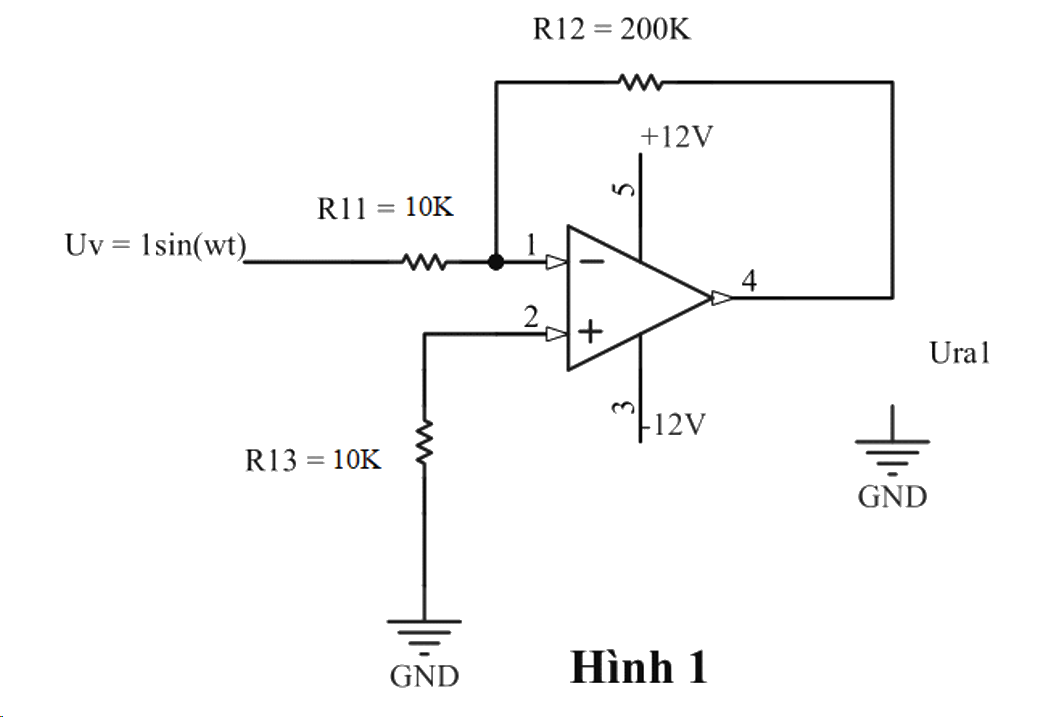
\includegraphics[width=0.9\linewidth]{screenshot001}
		\end{center}
		\vspace{1cm}
		\begin{flushleft}
			\color{red}\textbf{Câu 2: }\color{black} Tính và vẽ hình dạng điện áp $U_{ra2}$ của mạch khuếch đại cho ở hình 2
		\end{flushleft}
		\begin{center}
			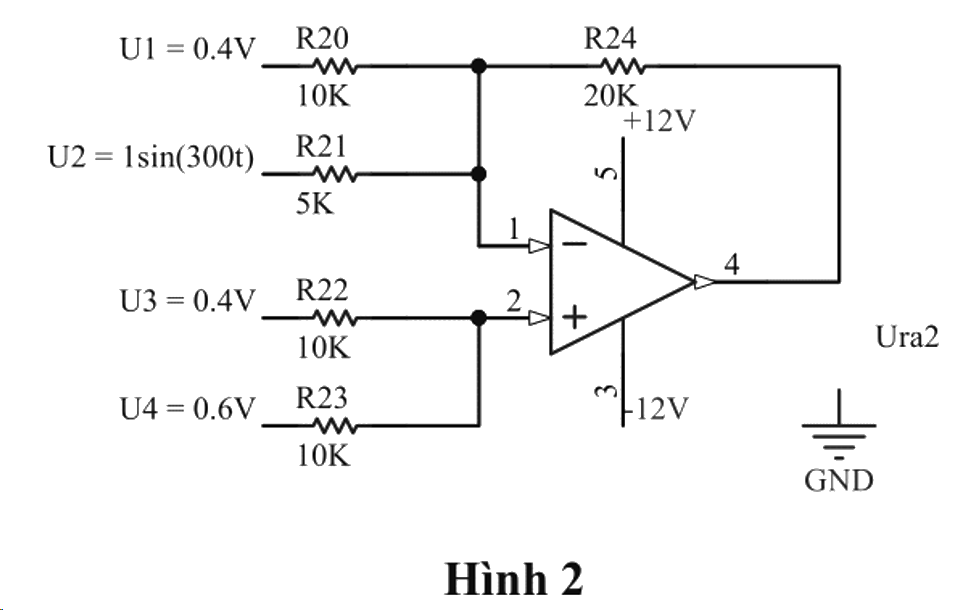
\includegraphics[width=0.9\linewidth]{screenshot002}
		\end{center}
		\vspace{1cm}
		\begin{flushleft}
			\color{red}\textbf{Câu 3: }\color{black} Cho mạch so sánh điện áp ở hình 3.Biết $+V_{s} = 11V , -V_{s} = -11V$
		\end{flushleft}
		
		a) Hãy xác định các điểm chuyển trạng thái và vẽ đặc tuyến $U_{ra}$ = f($U_{vao}$)
		
		b) Vẽ hình dạng của điện áp $U_{ra}(t)$ theo $U_{vao}(t)$
		\begin{center}
			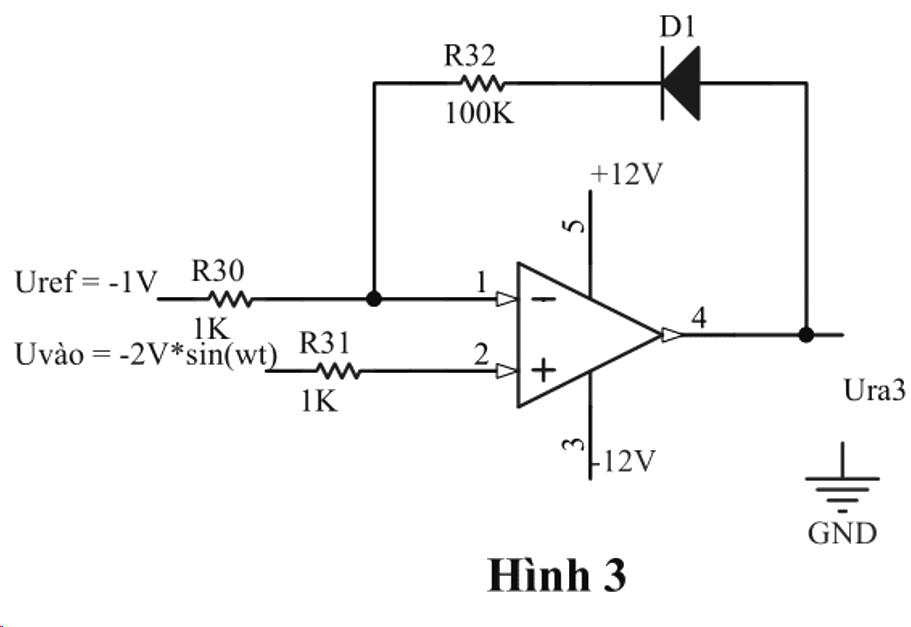
\includegraphics[width=0.9\linewidth]{screenshot003}
		\end{center}
		\vspace{1cm}
		\begin{flushleft}	
			\color{red}\textbf{Câu 4: }\color{black} Cho mạch chỉnh lưu chính xác ở hình 4
		\end{flushleft}
		
		a) Hãy xác định điểm bắt đầu chỉnh lưu và vẽ đặc tuyến $U_{ra} = f(U_{vao})$
		
		b) Vẽ hình dạng của điện áp $U_{ra}(t)$ theo $U_{vao}(t)$
		
		\begin{center}
			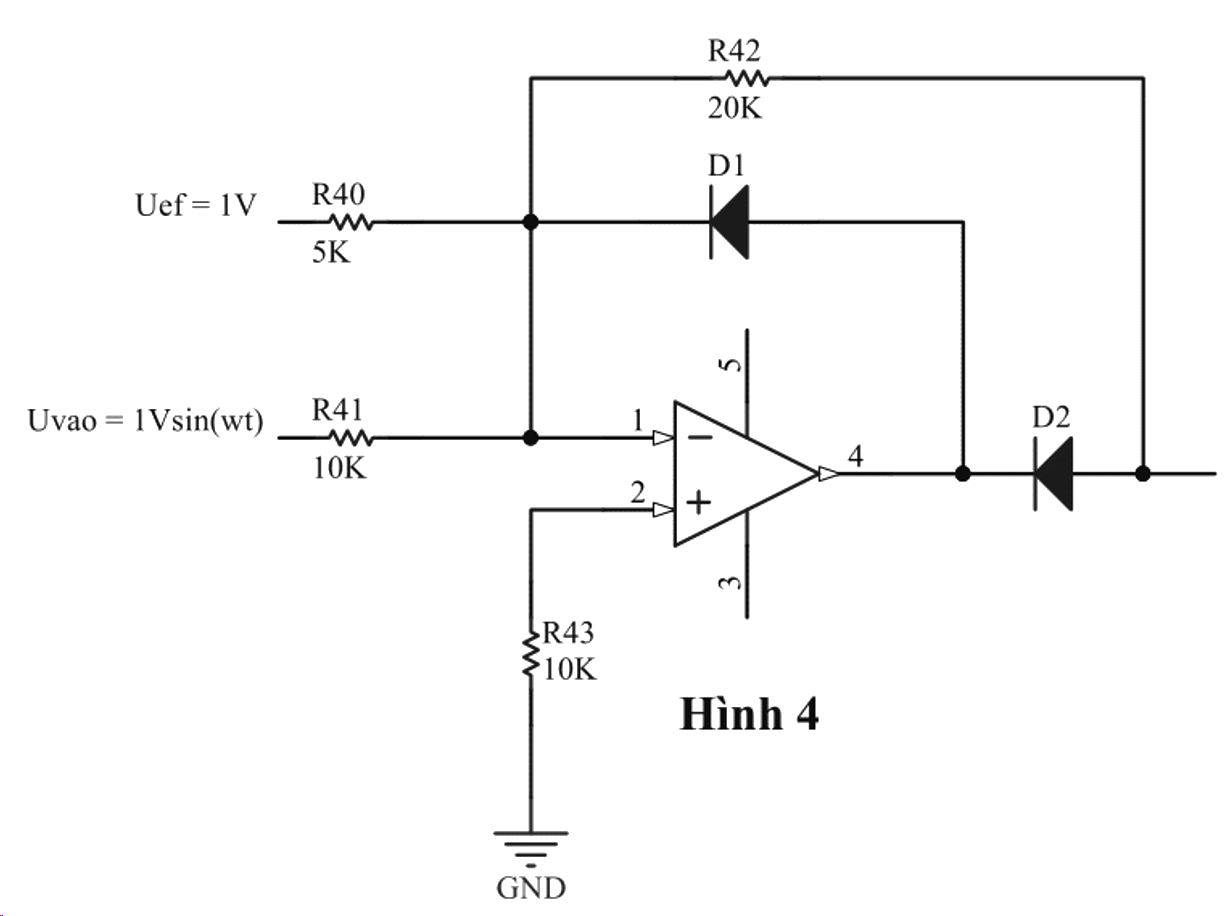
\includegraphics[width=0.9\linewidth]{screenshot004}
		\end{center}
		\vspace{1cm}
		\begin{flushleft}
			\color{red}\textbf{Câu 5: }\color{black} Cho mạch tích phân ở hình 5. Hãy vẽ hình dạng điệp áp $U_{ra5}$ trong thời gian 2s. Biết giá trị ban đầu $U_{ra5}(t = 0) = +10V$
		\end{flushleft}
		\begin{center}
			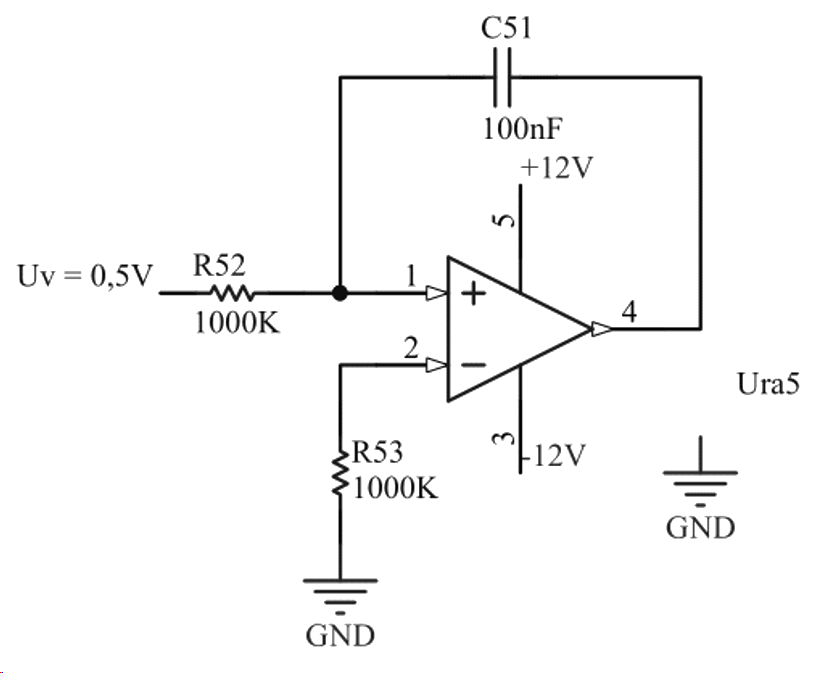
\includegraphics[width=0.9\linewidth]{screenshot005}
		\end{center}
		
		\newpage
%	\end{multicols}
	
	
\end{document}